%\documentclass[aspectratio=169]
\documentclass[aspectratio=169,xcolor=dvipsnames]{beamer}
%\usetheme{Copenhagen}
\usetheme{Madrid}
\setbeamertemplate{navigation symbols}{}
%\setbeamertemplate{footline}{}
\usecolortheme[named=Green]{structure}

\usepackage[utf8]{inputenc}

\usepackage{graphicx}         
\graphicspath{ {./Pictures/} }
\usepackage{amsmath}
\usepackage{amsfonts}
\usepackage{amssymb}
\usepackage{amsthm}
\usepackage{mathtools}
\usepackage{commath}
\usepackage{multimedia}
\usepackage{subcaption}
\usepackage{media9}
\addmediapath{Animations/}
\newcommand{\Sta}{y}
\newcommand{\Adj}{p}
\newcommand{\Con}{u}
\begin{document}

\title[]{{\huge PDE-Constrained Optimization \\for Multiscale Particle Dynamics} \\ With Industrial Applications}
\author[Jonna Roden (University of Edinburgh)]{Jonna Roden}
\institute[]{Supervision by Dr Ben Goddard and Dr John Pearson\\ University of Edinburgh, MIGSAA}
\date{}
\titlepage
 
 



\begin{frame}
\frametitle{PDE-Constrained Optimization \footnotesize{for Multiscale Particle Dynamics,\\ with Industrial Applications}}

\begin{align*}
\min_{\Sta,u} \quad \frac{1}{2}||&{\Sta(x,t)- \hat{\Sta}(x,t)}||_{L_2(\Omega \times (0,T))}^2 + \frac{\beta}{2} ||{\Con}(x,t)||_{L_2(\Omega \times (0,T))}^2\\
\\
\text{subject to} &\text{:}
\\
\partial_t \Sta(x,t) &=\nabla^2 \Sta(x,t) +\Con(x,t) + \alpha \nabla \cdot\int_\Omega \Sta(x,t) \Sta(x',t) \nabla V_2(|x-x'|)dx' \\
  \Sta(x,0)&=\Sta_0\\
  \\
  &+\text{ Boundary Conditions for $\Sta$.}
\end{align*}

\end{frame}

\begin{frame}
\frametitle{PDE-Constrained Optimization \footnotesize{for Multiscale Particle Dynamics,\\ with Industrial Applications}}
A non-standard solution strategy is needed because of the non-local term in the PDE:
\newline
\newline
\textbf{Pseudospectral Methods and Multiple Shooting}
\begin{itemize}
	\item Pseudospectral Methods lead to systems with small, dense matrices.
	\item Boundary Conditions easily applied within existing framework (2DChebClass).
	\item IVP solver \& Interpolation.
	\item Spectral Accuracy.
\end{itemize}

\begin{columns}

\column{0.3\linewidth}
\textbf{Industrial Applications}
\begin{itemize}
	\item Brewing.
	\item Nano-filtration.
	\item ...
\end{itemize}
\column{0.7\linewidth}
	\vspace{-1cm}
	\begin{figure}
		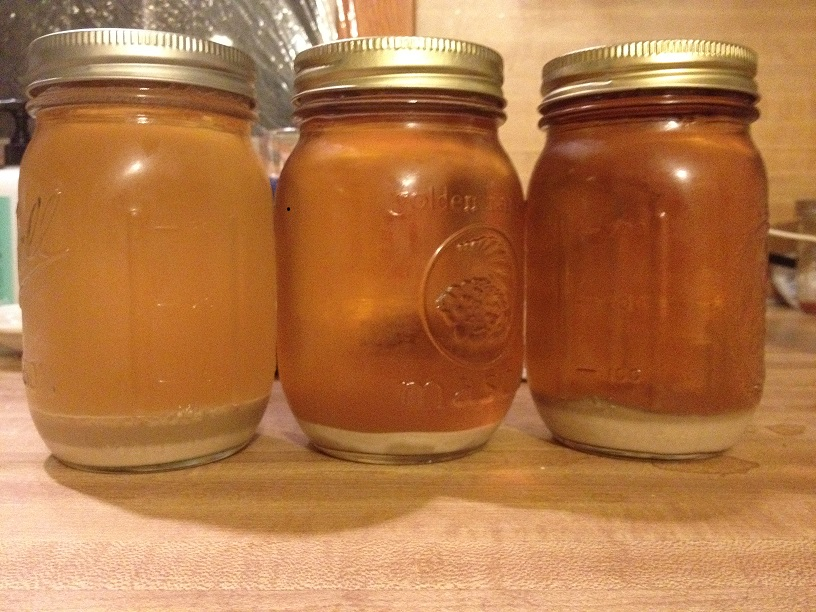
\includegraphics[width=3cm]{beer.jpg} \ \ \ \ \ \ \ \ 
		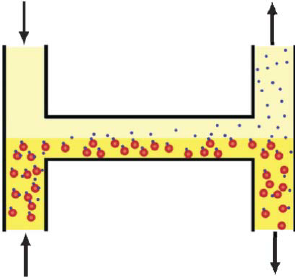
\includegraphics[width=3cm]{Microfilter.png}
		\caption{Brewing and Nano-filtration}
	\end{figure}
\end{columns}
\end{frame}




\end{document}
